\documentclass[11pt]{article}
\title{\LARGE{\bf \textsf{CS550: Massive Data Mining and Learning}}\\ {\bf \textsf{Homework 2}}}
\author{Christos Mitropoulos - cm1012 \\ email \href{mailto:c.mitro@rutgers.edu}{c.mitro@rutgers.edu} \\\\ Github repository:\\ \href{https://github.com/CMitropoulos/MassiveDataMining/tree/master/Homework2}{https://github.com/CMitropoulos/MassiveDataMining/tree/master/Homework2}}
\date{}
\usepackage{fullpage}
\usepackage{url}
\usepackage{listings}
\usepackage{amsmath}
\usepackage{hyperref}
\usepackage{comment}
\usepackage{graphicx}
\begin{document}
\begin{titlepage}
\maketitle
\end{titlepage}

\pagebreak[4]
\begin{center}
\LARGE{\bf \textsf{Submission Instructions}} \\*[4ex]
\end{center}

\textbf{Assignment Submission } Include a signed agreement to the Honor Code with this assignment. Assignments are due at 11:59pm. All students must submit their homework via Sakai. Students can typeset or scan their homework. Students also need to include their code in the final submission zip file. Put all the code for a single question into a single file. 
\\
\\
\textbf{Late Day Policy } Each student will have a total of {\em two} free late days, and for each homework only one late day can be used. If a late day is used, the due date is 11:59pm on the next day.
\\
\\
\textbf{Honor Code } Students may discuss and work on homework problems in groups. This is encouraged. However, each student must write down their solutions independently to show they understand the solution well enough in order to reconstruct it by themselves.  Students should clearly mention the names of all the other students who were part of their discussion group. Using code or solutions obtained from the web is considered an honor code violation. We check all the submissions for plagiarism. We take the honor code seriously and expect students to do the same. 

\vfill
\vfill

Discussion Group (People with whom you discussed ideas used in your answers): \\\\\\
On-line or hardcopy documents used as part of your anwsers: \\\\\\
\vfill

\vfill

I acknowledge and accept the Honor Code.\\*[3ex]
\bigskip
\textit{(Signed)} Christos Mitropoulos - CM

If you are not printing this document out, please type your initials above.

\vfill
\vfill

\pagebreak[4]
\section*{Answer to Question 1(a)}
Yes,$MM^{T} and$ $M^{T}M$ are symmetric, square and real.\\
\begin{itemize}
\item Symmetric: $(MM^{T})^T = MM^{T}$ and $(M^{T}M)^T = M^{T}M$
\item Square: Assuming M is a pxq matrix, when M is multiplied by its transpose, a qxp matrix, the result is a square matrix with rxr dimensions.
\item Real: Since M is a real matrix, the product of M and its transpose will also be real.
\end{itemize}
\section*{Answer to Question 1(b)}
Let's assume that e is the eigenvector of $MM^T$ and $\lambda$ its corresponding eigen value so that, $MM^T(e) = \lambda (e)$.
Multiply both sides of equation by $M^T$and the result is 
$M^TMM^Te = \lambda (e)$ which can be reduced to 
$M^TM(M^Te) = \lambda(M^Te)$.Therefore, the eigenvalue of $M^TM = \lambda$ too. However, the eigenvector is $M^Te$ which is different from the eigenvector of $MM^T$ which is e.
\section*{Answer to Question 1(c)}
$M^TM = Q\Lambda Q^T$
\section*{Answer to Question 1(d)}
$M^TM = (U \Sigma V^T)^T U \Sigma V^T = V\Sigma^T U^T U\Sigma V^T =   V\Sigma^T \Sigma V^T =  V\Sigma^2 V^T$
\section*{Answer to Question 1(e)(a)}
U = array([[-0.27854301,  0.5       ],
       [-0.27854301, -0.5       ],
       [-0.64993368,  0.5       ],
       [-0.64993368, -0.5       ]] \\
$\Sigma$ =  array([ 7.61577311,  1.41421356] \\
V = array([[-0.70710678, -0.70710678],
       [-0.70710678,  0.70710678]])

\section*{Answer to Question 1(e)(b)}
58.0: [ 0.70710678  0.70710678]\\
2.0: [-0.70710678  0.70710678]
\section*{Answer to Question 1(e)(c)}
The matrix of eigenvectors is equivalent to the V if we reorder the columns based on the ordering of singular values.
\section*{Answer to Question 1(e)(d)}
The singular values of M are square roots of the eigenvalues of $M^TM$
\section*{Answer to Question 2(a)}
We need to prove that: 
$\sum_{i=1}^{n}\sum_{j=1}^{n}{M_{ij}r_j} = \sum_{i=1}^{n}{r_i} $ \\
However, $\sum_{i=1}^{n}{M_{ij}} =1  $ for each j, thus this is True.
\section*{Answer to Question 2(b)}
Let's calculate w(r') first. \\
$ w(r') = \sum_{i=1}^{n}\beta \sum_{j=1}^{n}{M_{ij}r_j} + \sum_{i=1}^{n}(1-\beta)/n$ \\
The second term sums to 1 - $\beta$ and from (a) the first term sums to $\beta\sum_{j=1}^{n}r_j $\\
Thus, $w(r') =\beta w(r) +1-\beta $. Setting $ w(r) = w(r')= x$ and solving for x, we get that the equation is true if and only if $ w(r) = w(r')= 1$
\section*{Answer to Question 2(c)(a)}
The equation is $ r_i' = \beta\sum_{j=1}^{n}M_{ij}r_j + (1-\beta)/n + (\beta/n)\sum_{dead_j}r_j $ 
\section*{Answer to Question 2(c)(b)}
Summing over $M_{ij}$ as we did in 2(a) we get $w(r') = \beta \sum_{livej}r_j + 1 - \beta + \beta \sum_{deadj}r_j. $\\
The first and last terms give us $\beta w(r)$ which is actually $\beta$ since w(r) is supposed to be 1. Thus, the right side is 1 as well.

\section*{Answer to Question 3(a)}
TOP 5:\\
('ID: ', 53, ',score: ', array([ 0.0357312]))\\
('ID: ', 14, ',score: ', array([ 0.03417091]))\\
('ID: ', 40, ',score: ', array([ 0.03363009]))\\
('ID: ', 1, ',score: ', array([ 0.03000598]))\\
('ID: ', 27, ',score: ', array([ 0.02972014]))\\
\section*{Answer to Question 3(b)}

BOTTOM 5:\\
('ID: ', 85, ',score: ', array([ 0.00340969]))\\
('ID: ', 59, ',score: ', array([ 0.00366986]))\\
('ID: ', 81, ',score: ', array([ 0.00369535]))\\
('ID: ', 37, ',score: ', array([ 0.0038082]))\\
('ID: ', 89, ',score: ', array([ 0.00392247]))\\

\section*{Answer to Question 4(a)}
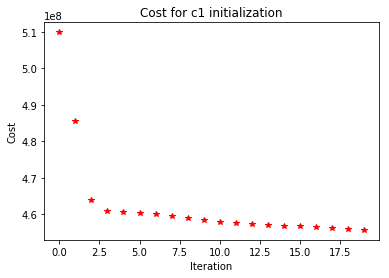
\includegraphics{c1_cost} \\
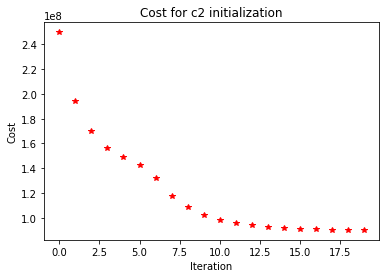
\includegraphics{c2_cost} 

\section*{Answer to Question 4(b)}
The cost for c2 initialization drops faster, since the clusters are distributed far apart. Since there is less overlap between clusters, true clusters will be split less often. We reach convergence faster.
The percentage improvement after 10 iterations for c1 initialization is 0.10 and for c2 initialization is 0.59.
\end{document}

